\documentclass[10.7pt,]{article}

%in the preamble
%--------------------------------
\usepackage[
backend=biber,
style=numeric-comp,
sorting=none,
minbibnames=3,
]{biblatex}

% supress pp. and add a semi-colon
\DefineBibliographyStrings{english}{%
  page             = {:\ifbibliography{}{}},
  pages            = {:\ifbibliography{}{}},
} 
\renewcommand*{\ppspace}{}

% Supresses In in the bibliographics
\renewbibmacro{in:}{}

\renewbibmacro*{journal+issuetitle}{%
  \usebibmacro{journal}%
  \setunit*{\addspace}%
  \iffieldundef{series}
    {}
    {\newunit
     \printfield{series}%
     \setunit{\addspace}}%
  \setunit{\addspace}%
  \usebibmacro{issue+date}%
  \setunit{\addcolon\space}%
  \usebibmacro{issue}%
  \setunit{\addsemicolon}%
  \usebibmacro{volume+number+eid}%
  \newunit}

\DeclareFieldFormat[article,periodical]{number}{\mkbibparens{#1}}
\renewbibmacro*{volume+number+eid}{%
  \printfield{volume}%
  \printfield{number}%
  \setunit{\addcomma\space}%
  \printfield{eid}}

\renewbibmacro*{issue+date}{%
  \iffieldundef{issue}
    {\usebibmacro{date}}
    {\printfield{issue}%
     \setunit*{}%
     \usebibmacro{date}}%
  \newunit}
  
\renewcommand*{\bibpagespunct}{}
 
\addbibresource{literature.bib}
%--------------------------------
%\usepackage[numbers]{natbib}
%\bibliographystyle{dcu}
%\bibpunct{[}{]}{;}{n}{}{,}


\usepackage[letterpaper, margin=2.54cm, top=2.54cm]{geometry}
\usepackage{lmodern}
\usepackage{authblk} % To add affiliations to authors
\usepackage{amssymb,amsmath}
\usepackage{wrapfig}
\usepackage{graphicx,grffile}
\usepackage[labelfont=bf,labelsep=period]{caption}
\usepackage{ifxetex,ifluatex}
\usepackage{bm}
\usepackage{array, boldline, makecell, booktabs}
\usepackage{multirow}


%\usepackage{fixltx2e} % provides \textsubscript
\ifnum 0\ifxetex 1\fi\ifluatex 1\fi=0 % if pdftex
  \usepackage[T1]{fontenc}
  \usepackage[utf8]{inputenc}
\else % if luatex or xelatex
  \ifxetex
    \usepackage{mathspec}
  \else
    \usepackage{fontspec}
  \fi
  \defaultfontfeatures{Ligatures=TeX,Scale=MatchLowercase}
    \setmainfont[]{Arial Narrow}
    \setsansfont[]{Century Gothic}
    \setmonofont[Mapping=tex-ansi]{Consolas}
\fi
% use upquote if available, for straight quotes in verbatim environments
\IfFileExists{upquote.sty}{\usepackage{upquote}}{}
% use microtype if available
\IfFileExists{microtype.sty}{%
	\usepackage{microtype}
	\UseMicrotypeSet[protrusion]{basicmath} % disable protrusion for tt fonts
}{}



%==============================
% Customization to make the output PDF 
% look similar to the MS Word version
%==============================
% To prevent hyphenation
\hyphenpenalty=10000
\exhyphenpenalty=10000

% To set the sections font size
\usepackage{sectsty}
\allsectionsfont{\fontsize{11}{11}\selectfont}
\sectionfont{\fontsize{14}{14}\selectfont}
\subsectionfont{\bfseries\fontsize{13}{13}\selectfont}
\subsubsectionfont{\bfseries\fontsize{11}{11}\selectfont}
%\subsubsectionfont{\normalfont}

% Spacing
\usepackage{setspace}

\usepackage{xcolor}

\usepackage{dsfont}
\usepackage{amsmath,amssymb}
\DeclareMathOperator*{\argmax}{arg\,max}
\DeclareMathOperator*{\argmin}{arg\,min}


% No new line after subsubsection
\makeatletter
%\renewcommand\subsubsection{\@startsection{subsubsection}{3}{\z@}%
%	{-3.25ex\@plus -1ex \@minus -.2ex}%
%    {-1.5ex \@plus -.2ex}% Formerly 1.5ex \@plus .2ex
%    {\normalfont}}
%\makeatother

% To set the doc title font
\usepackage{etoolbox}
\makeatletter
\patchcmd{\@maketitle}{\LARGE}{\bfseries\fontsize{15}{16}\selectfont}{}{}
\makeatother

% No page numbering
\pagenumbering{gobble}

\makeatletter
\def\maxwidth{\ifdim\Gin@nat@width>\linewidth\linewidth\else\Gin@nat@width\fi}
\def\maxheight{\ifdim\Gin@nat@height>\textheight\textheight\else\Gin@nat@height\fi}
\makeatother

% Scale images if necessary, so that they will not overflow the page
% margins by default, and it is still possible to overwrite the defaults
% using explicit options in \includegraphics[width, height, ...]{}
\setkeys{Gin}{width=\maxwidth,height=\maxheight,keepaspectratio}
\setlength{\parindent}{0pt}
\setlength{\parskip}{6pt plus 2pt minus 1pt}
\setlength{\emergencystretch}{3em}  % prevent overfull lines
\providecommand{\tightlist}{%
  \setlength{\itemsep}{0pt}\setlength{\parskip}{0pt}}
\setcounter{secnumdepth}{0}
% Redefines (sub)paragraphs to behave more like sections
\ifx\paragraph\undefined\else
\let\oldparagraph\paragraph
\renewcommand{\paragraph}[1]{\oldparagraph{#1}\mbox{}}
\fi
\ifx\subparagraph\undefined\else
\let\oldsubparagraph\subparagraph
\renewcommand{\subparagraph}[1]{\oldsubparagraph{#1}\mbox{}}
\fi
%==============================
\usepackage{hyperref}
\hypersetup{
	unicode=true,
	pdftitle={My Cool Title Here},
	pdfauthor={Author One, Author Two, Author Three},
	pdfkeywords={keyword1, keyword2},
	pdfborder={0 0 0},
	breaklinks=true
}
\urlstyle{same}  % don't use monospace font for urls

% Keywords command
\providecommand{\keywords}[1]
{
  \small	
  \textbf{Key words---} #1
}
%==============================
\title{Not So Weak-PICO: Leveraging weak supervision for Participants, Interventions, and Outcomes recognition for systematic review automation}
\date{}
\author[ ] {
    % Authors
    \bf\fontsize{13}{14}\selectfont
    Anjani Dhrangadhariya\textsuperscript{\rm 1, 2},
    Henning M\"uller \textsuperscript{\rm 1, 2}
}
\affil[1]{Informatics Institute, University of Applied Sciences Western Switzerland (HES-SO), Sierre, Switzerland}
\affil[2]{University of Geneva (UNIGE), Geneva, Switzerland}
\affil[*]{Corresponding author: Anjani Dhrangadhariya, Rue de Technopôle 3, Informatics Institute, University of Applied Sciences Western Switzerland (HES-SO), 3960 Sierre, Switzerland; anjani.dhrangadhariya@hevs.ch; +41 58 606 90 03}
%==============================
\begin{document}
\maketitle
%==============================
\doublespacing
%==============================

Word count: 3981

\clearpage
\section{\textbf{ABSTRACT}}
\label{abstract}
%==============================
% Note: Abstract is limited to 250 words
%==============================
\textbf{Objective:}
%PICO (Participants, Interventions, Comparators, Outcomes) analysis is vital but time-consuming for conducting systematic reviews (SRs).
%Supervised machine learning can help fully automate it, but a lack of large annotated corpora limits the quality of automated PICO recognition systems.
%The largest currently available PICO corpus is manually annotated, which is an approach that is often too expensive for the scientific community to apply.
%Depending on the specific SR question, PICO criteria are extended to PICOC (C-Context),  PICOT (T-timeframe), and PIBOSO (B-Background, S-Study design, O-Other), meaning the static hand-labelled corpora need to undergo costly re-annotation as per the downstream requirements.
%We aim to test the feasibility of designing a weak supervision system to extract these entities without hand-labelled data.
To test the feasibility of PICO (Participants, Interventions, Comparators, Outcomes) entity extraction using weak supervision and natural language processing.
\textbf{Methodology:}
%We decompose PICO spans into its constituent entities and re-purpose multiple medical and non-medical ontologies and expert-generated rules to obtain multiple noisy labels for these entities.
%These labels generated using several sources are then aggregated using simple majority voting and generative modelling approaches.
%The resulting programmatic labels are used as weak signals to train a weakly-supervised discriminative model and observe performance changes.
%We explore mistakes in the currently available PICO corpus that could have led to inaccurate evaluation of several automation methods.
We re-purpose $>127$ medical and non-medical ontologies and expert-generated rules to obtain multiple noisy labels for PICO entities in the EBM-PICO corpus.
These noisy labels are aggregated using simple majority voting and generative modelling to get consensus labels.
The resulting probabilistic labels are used as weak signals to train a weakly-supervised discriminative model and observe performance changes.
We explore mistakes in the EBM-PICO that could have led to inaccurate evaluation of previous automation methods.
\textbf{Results:}
%We present Weak-PICO, a weakly-supervised PICO entity recognition approach using medical and non-medical ontologies, dictionaries and expert-generated rules.
%Our approach does not use hand-labelled data.
In total, 4,081 randomized clinical trials (RCT) were weakly labelled to train the weakly-supervised models and compared against full supervision.
The models were separately trained for PICO entities and evaluated on the EBM-PICO test set.
A weakly-supervised approach combining ontologies and expert-generated rules outperformed full supervision for the participant entity by 1.71\% macro-F1.
Error analysis on the EBM-PICO subset revealed 18-23\% erroneous token classifications.
\textbf{Discussion:}
Automatic PICO entity extraction accelerates the writing of clinical systematic reviews that commonly use PICO information to filter health evidence.
However, PICO extends to more entities - PICOS (S-Study type and design), PICOC (C-Context), and PICOT (T-timeframe) for which labelled datasets are unavailable.
In such cases, the ability to use weak supervision overcomes the expensive annotation bottleneck.
\textbf{Conclusion:}
%Weak supervision using weak-PICO for PICO entity recognition has encouraging results, and the approach can potentially extend to more clinical entities readily.
We show the feasibility of weakly-supervised PICO entity extraction using freely-available ontologies and heuristics without manually annotated data. Weak supervision has encouraging performance compared to full supervision but requires careful design to outperform it. 


\keywords{Weak supervision, Machine learning, Information extraction, Evidence-based Medicine}


%
\clearpage
% Full paper is limited to 4000 words (approx. 14.6 pages)
%
%==============================
\section{\textbf{INTRODUCTION}}\label{introduction}
%==============================
%
Systematic reviews (SR) are an evidence-based practice of answering clinical questions using a transparent and quantitative approach.
The reviewers must collect as many candidate publications as possible, identify the relevant publications, and integrate their results via statistical meta-analysis.
A clinical SR question is typically formulated using the PICO framework (Participants, Interventions, Comparators, Outcomes), e.g., ``Will aerobic exercise (\textbf{Intervention}) improve fatigue (\textbf{Outcome}) in cancer patients (\textbf{Participant}) compared to usual care (\textbf{Comparator})?''.
A publication is only relevant for answering a question if it studies the question-relevant participants, interventions (comparators) and outcomes.\cite{uman2011systematic} 
Manually analyzing PICO information from thousands of publications to gauge its relevance often takes 2-8 months of two medical experts' time for a single SR.\cite{borah2017analysis}
The process can be automated using machine learning (ML) by directly pointing the human reviewers to the correct text chunks describing PICO, facilitating quick decision-making for the study's relevance.



Supervised ML requires hand-labelled data, but hand-labelling PICO information requires experts with combined medical and informatics skills, which is expensive and time-consuming in terms of intensive annotator training and the actual annotation.
Labelling PICO is tricky because of the high disagreement between human annotators on the exact spans constituting PICO, leading to human errors in hand-labelled corpora.\cite{brockmeier2019improving}
Some studies examine the errors in the publicly-available EBM-PICO benchmark.\cite{nye2018corpus,abaho2019correcting,lee2019study}
More importantly, depending upon the clinical SR question, PICO criteria extend to PICOS (S-Study design), PICOC (C-Context), PICOT (T-timeframe), \textit{etc}.\cite{riva2012your,methley2014pico,uman2011systematic}
Hand-labelled datasets are static and prohibit quick manual re-labelling in case of human errors or when a downstream task requires new entities.
This annotation bottleneck has pivoted attention towards weakly supervised (WS) learning that relies on programmatic labelling sources to obtain training data.
Programmatic labelling is quick and allows efficient modifications to the training data labels per the downstream application changes.



Weakly-supervised learning has demonstrated strengths for clinical document classification and relation extraction, but clinical entity extraction tasks have heavily relied on fully supervised (FS) approaches.\cite{meng2018weakly,wang2019clinical,mintz2009distant,elangovan2020assigning,weber2020pedl,mallory2020extracting}
Despite the availability of UMLS (Unified Medical Language System), a large compendium of medical ontologies, which can be re-purposed for weak entity labelling, it has not been extensively applied to clinical entity labelling.\cite{humphreys1998unified}
Several legacy clinical applications are also supported by rule-based \textit{if-else} systems relying on keyword cues that aid weak labelling.\cite{friedlin2008software,kim2017extracting,yang2015automatic}
With so many weak labelling sources available, the challenge for weak supervision is efficiently aggregating these sources of varying accuracy.



Data programming is a domain-agnostic generative modelling approach combining multiple weak labelling sources and estimating their accuracies.
The effectiveness of data programming for biomedical entity recognition has been explored by Fries \textit{et al.} in their Trove system.\cite{fries2021ontology}
However, Trove only explores well-defined entities like chemical, disease, disorder and drug classes.
PICO categories are highly compositional spans by definition, fuzzier in comparison and much more intricate in that they can be divided into subclasses.
A shortcoming of span extraction is that even after a machine points a human reviewer to the correct PICO span, the reviewer requires to manually read and understand its finer aspects to screen the study for relevance.
Span extraction hence leads to semi-automation but hinders full-automation.
The entity recognition approach to PICO is more challenging than the entity recognition approach to disease or chemical names which are more or less standardized.
PICO terms are not standard, and even the experts disagree on the exact tokens constituting them.\cite{brockmeier2019improving}
Weakly-supervised PICO entity recognition has not garnered as much attention as supervised span recognition.
As far as our knowledge goes, only two studies exist for weakly-supervised PICO recognition.
One of these approaches only explores distant supervision for intervention extraction using a single labelling source.\cite{dhrangadhariya2022distant}
The other approach studies weak supervision for PICO span extraction but still utilizes some supervised annotation signals about whether a sentence includes PICO information.\cite{liu2021sent2span}
%The other relies on a single source of programmatic labelling and focuses on PICO spans and sentences rather than entities.\cite{liu2021sent2span}



The challenges to developing weak supervision approaches to PICO entity recognition are first defining the subclasses within PICO spans and then mapping several available ontologies and terminologies to these.
The next challenge is developing weakly-supervised classifiers by optimally combining ontologies and evaluating their performance compared to full supervision.
Another challenge is developing higher-cost expert-generated rules corresponding to these subclasses to aid ontology classifiers and evaluate their combined performance.
We also identified limitations in the currently available EBM-PICO training set and corrected them in the EBM-PICO test set for reliable evaluation of the WS approaches.
Our work demonstrates the feasibility of using weak supervision for PICO entity extraction using the EBM-PICO benchmark and shows how weak supervision overtakes full supervision in certain instances.
%We show how using only ontology-dependent classifiers vs combining them with expert-generated rules compares to fully-supervised extraction and, in some instances overtaking it.
%
%
%
%==============================
\section{METHODOLOGY}\label{methods}
%==============================
%
The birds-eye view of our approach is shown in Figure~\ref{fig:approach}.
%
\begin{figure}[ht]
\centering
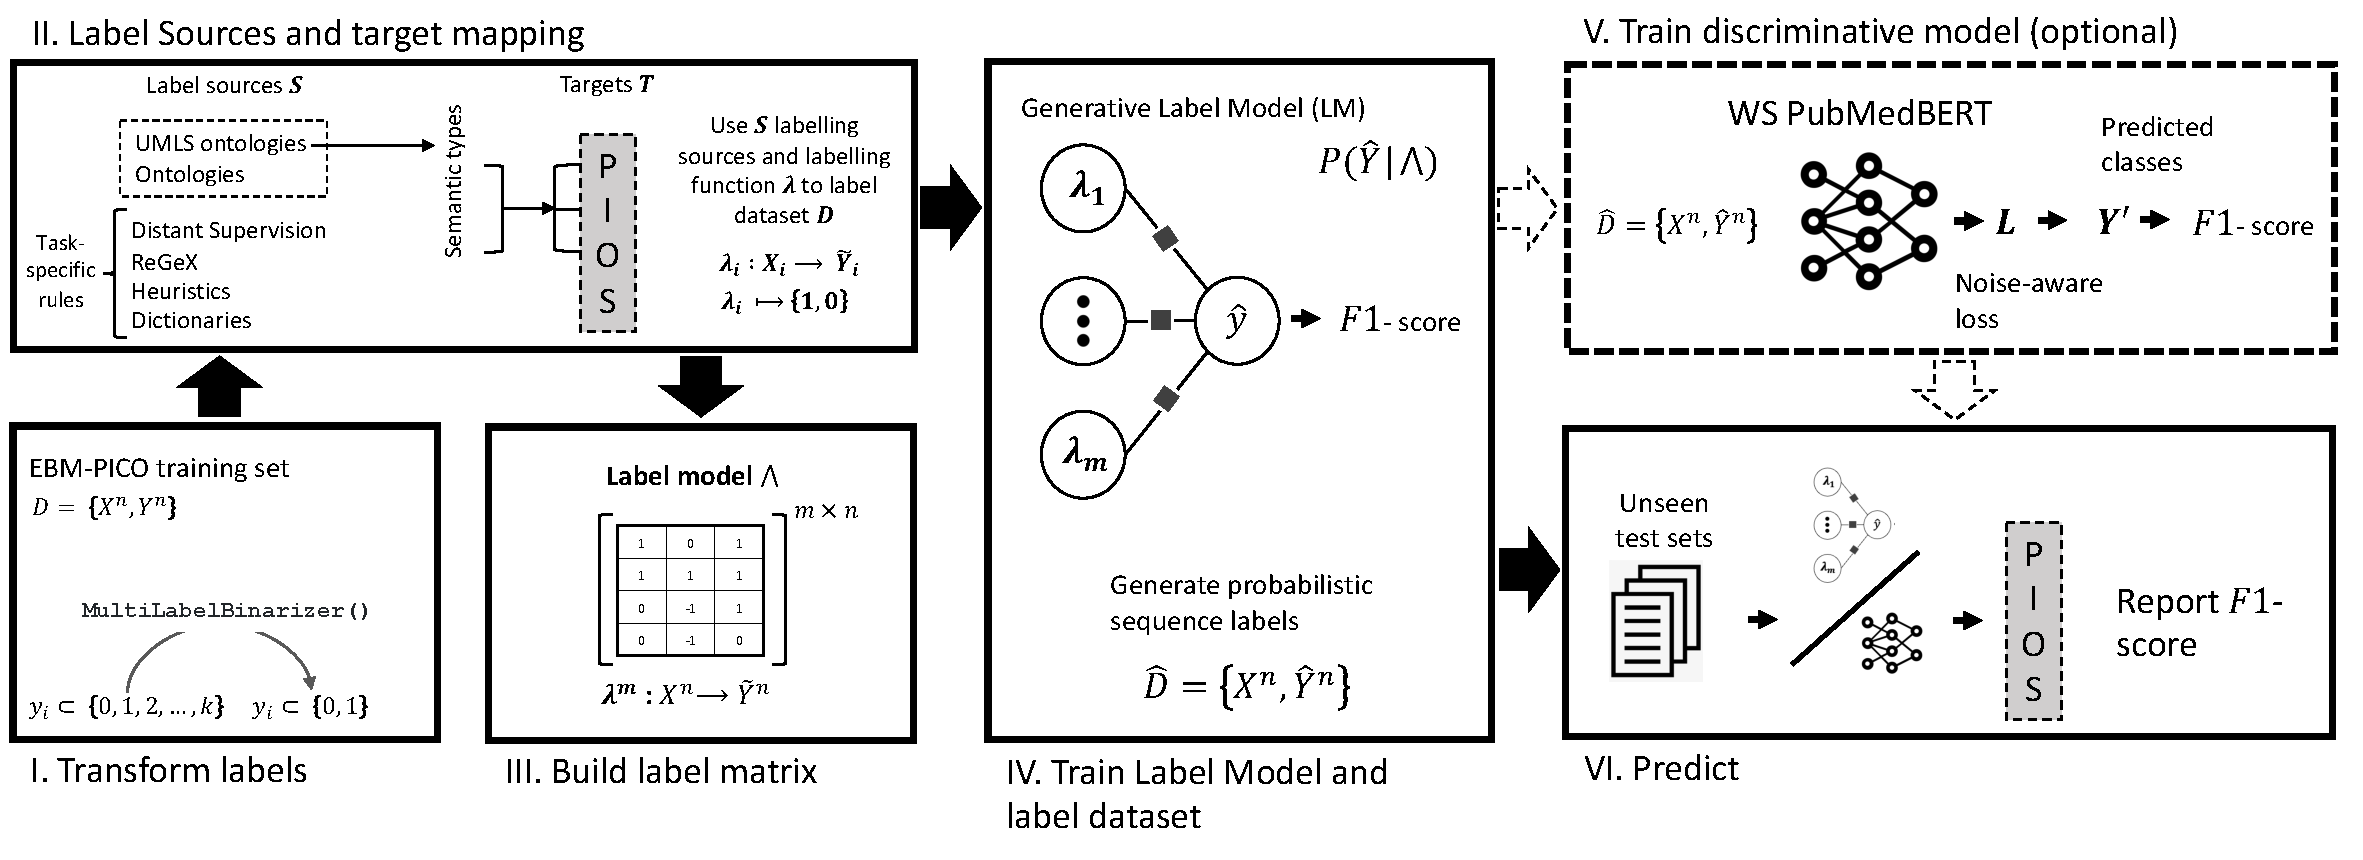
\includegraphics[width=0.98\textwidth]{figures/approach.pdf}
\caption{Weak PICO entity extraction approach: I) Multi-class labels in the EBM-PICO benchmark are binarized. II) Low-cost UMLS vocabularies are re-purposed as labelling sources, and experts design rules as high-cost labelling sources. III) Labelling functions map the training sequences to class labels using labelling sources resulting in an $m \times n$ label matrix. IV-V) The label matrix is used to train a generative model that outputs probabilistic labels that a downstream transformer model can use for entity recognition.}
\label{fig:approach}
\end{figure}
%
%==============================
\subsection{Datasets}\label{data}
%==============================
%
EBM-PICO is a widely used dataset with multi-level PICO annotations: span-level or coarse-grained and entity-level or fine-grained (see Table~\ref{tab:coarsefineconcept}).
Span-level annotations encompass the maximum information about each class.
Entity-level annotations cover the more fine-grained information at the entity level, with PICO classes further divided into more semantic subclasses.
The dataset comes pre-divided into a training set (n=4,933) annotated through crowd-sourcing and an expert annotated gold test set (n=191) for evaluation.\cite{nye2018corpus}

The EBM-PICO original paper and annotation guidelines caution about variable annotation quality\footnote{\url{https://www.ncbi.nlm.nih.gov/pmc/articles/PMC6174533/bin/NIHMS988059-supplement-Appendix.pdf}}.
Abaho \textit{et al.} developed a framework to post-hoc correct EBM-PICO outcomes annotation inconsistencies.\cite{abaho2019correcting}
Lee \textit{et al.} studied annotation disagreements suggesting variability across the annotators.\cite{lee2019study}
Low annotation quality in the training dataset is excusable, but the errors in the test set can lead to faulty evaluation of the downstream ML methods.
We evaluate \textasciitilde1\% of the EBM-PICO training set tokens to gauge the possible reasons for the fine-grained labelling errors and use this exercise to conduct an error-focused PICO re-annotation for the EBM-PICO gold set.
The paper's first author, who has a master's in life science informatics and relevant experience in manual curation projects, carried out the re-annotation.


The dataset is pre-tokenized and did not require additional preprocessing except the addition of POS tags and token lemma using spaCy\footnote{\url{https://spacy.io/}}.
Multi-class fine-grained PICO annotations were binarized, i.e. a token label was reset to 1 if the token represented a fine-grained entity.
%
\begin{table}[h!]
\begin{center}
\begin{tabular}{| c | c | c | c |} 
\hline
 & P & I/C & O \\ 
\hline
0 & No label & No label & No label \\ 
1 & Age & Surgical & Physical \\ 
2 & Sex & Physical & Pain \\
3 & Sample size & Drug & Mortality \\
4 & Condition & Educational & Side effect \\
5 &  & Psychological & Mental \\
6 &  & Other & Other \\
7 &  & Control &  \\
\hline
\end{tabular}
\caption{\label{tab:coarsefineconcept} P (Participant), I (Intervention) and O (Outcome) represent the coarse-grained labels that are further divided into respective fine-grained labels. The table is taken from Nye \textit{et al.}\cite{nye2018corpus}}
\end{center}
\end{table}
%
%==============================
\subsection{Binary token labelling}\label{seq_lab}
%==============================
%
We consider automatic PICO entity labelling as a classical binary token labelling problem whereby a labeller maps an input sequence of $n$ text tokens, $ \bm{X} = (x_{1}, x_{2}, \dotso , x_{n} )$ to output sequence $\bm{Y} = (y_{1}, y_{2}, \dotso , y_{n} )$, where $y_{i} \subset y; y = \{1,0\} $ is the label for token $x_{i}$.
In weak supervision, $\bm{Y}$ is latent and should be estimated by aggregating several weak labellers of variable accuracy.
The estimates $\bm{\hat{Y}}$ of $\bm{Y}$ are assigned as probabilistic token labels of $\bm{X}$ leading to a weakly labelled dataset that can be used to train discriminative models.
%
%
%
%==============================
\subsection{Labeling functions}\label{lfs}
%==============================
%
In a binary token labelling task, a labeller, also called a labelling function (LF) is a weak classifier $\lambda$ that uses domain-specific labelling sources $\bm{S}$ and some logic to emit binary token labels $ \widetilde{\bm{Y_{i}}}$ where $ \widetilde{y} \in \{-1, 0, +1\}$ for a subset of input $\bm{X_{i}}$ tokens.
An LF designed for a particular target class $t \in \bm{T}$ (here; $\bm{T} \subset \{ Participant, Intervention, Outcome \} $) should output  $1$ for the positive token class label, $0$ for the negative token class label, and abstain ($-1$) on the tokens where it is uncertain $\lambda \mapsto \{-1, 0, +1\}$.
We designed three LF types depending on the types of labelling sources.
1) The ontology LFs for a target class take a dictionary of terminologies with each terminology mapped to one of $y \subset \{0, +1\} $ token target labels.
Any labelling function using terminologies used string matching as the labelling heuristic.
Relevant bigram word co-occurrences were used to account for fuzzy span matching from the terminologies.
A bigram was considered relevant for a vocabulary if it occurred $\geq25$ times in that vocabulary.
2) A ReGeX (regular expression) labelling function for a target class uses regular expression sources for both negative and positive token class $\{0, +1\}$ labels and abstains from the rest.
3) A heuristic labelling function is personalized for each target class and takes a generic regex pattern and specific POS (part-of-speech) tag signals.
Abbreviations in clinical studies are considered using a heuristics abbreviation identifier, and the identified abbreviations were mapped to their respective target classes.
Stopwords from Natural Language Tookit (NLTK)\footnote{\url{https://www.nltk.org}}, spaCy, Gensim\footnote{\url{https://radimrehurek.com/gensim/}}, and scikit learn\footnote{\url{https://scikit-learn.org}} were used to initialize negative token label templates.
%
%==============================
\subsection{Labelling sources}\label{lss}
%==============================
%
This section describes the labelling sources $\bm{S}$ used and their mapping to the PICO targets $\bm{T}$.
We used the 2021AB-full release of the UMLS Metathesaurus English subset with 223 vocabularies.
After removing non-English and zoonotic vocabulary and the vocabularies containing fewer than 500 terms, we remained with 127 vocabularies.\cite{humphreys1998unified}
Terms in the selected vocabularies were preprocessed by removing stopwords, numbers, and punctuation.
We use the following non-UMLS vocabularies: Disease Ontology (DO), Human Phenotype Ontology (HPO), Ontology of Adverse Events (OAE), Chemical entities of biological interest (ChEBI),  Comparative Toxicogenomics Database (CTD) - Chemical and Disease subclasses, Gender, Sex, and Sexual Orientation Ontology (GSSO), Chemotherapy Toxicities Ontology (ONTOTOX), Cancer Care: Treatment Outcomes Ontology (CCTOO), Symptoms Ontology (SYMP), Non-pharmacological Interventions Ontology (NPI), Nursing Care Coordination Ontology (NCCO).\cite{schriml2012disease,robinson2008human,he2014oae,de2010chemical,kronk2020development,geifman2011towards,rogier2021using,lin2018cancer,mohammed2012building,ninot2018definition}
ReGeX and heuristics like POS tag cues were used to capture recurring class-specific PICO patterns otherwise not captured by standardized terminologies.
Vocabularies are structured, standardized data sources that do not capture writing variations from clinical literature and custom-built ReGeX are restricted by either task or entity type.\cite{ratner2017snorkel,safranchik2020weakly}
We used distant supervision dictionaries created from the structured fields of clinicaltrials.gov (CTO) as described by Dhrangadhariya \textit{et al.}\cite{dhrangadhariya2022distant}
Principal investigators of the clinical study manually enter data in CTO, thereby incorporating large-scale writing variations.\cite{califf2012characteristics}
Hand-crafted dictionaries were generated using various web sources.
%
%
%
%==============================
\subsubsection{Sources to targets}\label{s2t}
%==============================
%
Along with the source $\bm{S}$ and the logic to map $S_{i}$ to token labels, an LF needs information about which target $T_{i}$ label and binary token class to map the source.
We report how the LF sources were mapped to PICO targets in this section.
UMLS 2021AB-full release contains 16,543,671 concept names, making direct concept to PICO target mapping impractical.
These concepts are organized under semantic type categories (e.g. disease, signs and symptoms, age group, etc.)\footnote{\url{https://www.nlm.nih.gov/research/umls/META3_current_semantic_types.html}}, which allows mapping these semantic categories to PICO targets invariably mapping the concepts from the vocabularies to target classes.\cite{mccray2001aggregating}
It is a challenging expert-led activity, though decomposing PICO into subclasses greatly helps map sources to a target.
A semantic category was marked $1$ to represent a positive token label for that target class or $0$ to represent a negative token label for that target class.
Non-UMLS vocabularies were obtained from NCBO bioportal\footnote{\url{https://bioportal.bioontology.org/}} and were chosen to be PICO target specific and assigned to a single label.
Structured fields from clinicaltrials.gov (CTO) were used to create target-specific distant supervision dictionaries.
The structured CTO field ``Condition or Disease'' was mapped to the participant target, and the ``Intervention/Treatment'' field was mapped to the intervention target.
The semi-structured ``Primary Outcome Measures'' and ``Secondary Outcome Measures'' fields were mapped to the outcome target.
The hand-crafted dictionaries for outcomes were designed using the official websites listing patient-reported outcome (PROM) questionnaires\footnote{\url{https://www.thoracic.org/members/assemblies/assemblies/bshsr/patient-outcome/}} and PROMs\footnote{\url{https://www.safetyandquality.gov.au/our-work/indicators-measurement-and-reporting/patient-reported-outcomes/proms-lists}}.
Other hand-crafted dictionaries were separately designed for participant gender and sexuality and intervention comparator terms.
%
%
%
%==============================
\subsection{LF aggregation}\label{lms}
%==============================
%
Depending upon the number of sources $\bm{S}$ for each $\bm{T}$, we had several LFs. 
Each LF $ \lambda_{i} \in \bm{\Lambda^{m}}; \bm{\Lambda} = \{\lambda_{1}, \lambda_{2}, \dotso, \lambda_{m} \} $ maps a subset of inputs $\bm{X^{n}}$ to output sequence $ \widetilde{\bm{Y^{n}}}$ with labels $\widetilde{y} \in \{-1, 0, +1\}$ yielding a label matrix $ \lambda \subset \{-1, 0, +1\}^{m \times n}$.
The weakly-generated labels might have conflicts and overlaps and are generally noisy.
These LFs can be ensembled using the majority vote (MV) rule, where a token label is elected only when a majority of $\lambda_{i}$ vote for it.
Ties and abstains lead to the selection of the majority label.
%
\begin{equation}
\bm{\hat{Y}_{MV}} = \max_{{y \subset \{ 0, 1 \} }} \sum_{i=1}^{m} \mathds{1} (\lambda_{i} = y_{i})
\end{equation}
%
However, MV considers each labelling function as conditionally independent and does not consider the variable accuracies of different labelling sources weighing them equally.
Snorkel implements data programming paradigm into the label model (LM) that re-weights and aggregates labelling functions into probabilistic labels $\hat{y_{i}}$.
To do this, the label model trains a generative model $ \bm{P} ( \Lambda , Y )$ to estimate LF accuracies $\theta_{j}$ using stochastic gradient descent to minimize log loss in the absence of labelled data.\cite{ratner2017snorkel,dunnmon2020cross}
Even though the ground truth is not observable to estimate accuracies, they can be estimated using observed agreement and disagreement rates between labelling function pairs $ \lambda_{i}, \lambda_{j}$ in $\Lambda$.
Generative modeling ultimately results into token label probablities $\bm{\hat{Y}}$ for label classes $ \{ 0, 1\} $.
GridSearch was used to fine-tune the label model parameters using the hand-labelled validation set from the EBM-PICO.
The parameters are listed in the Experimental details section of the supplementary material.
Once we have the pseudo-labels generated by majority voting or the label model, these could be used to train a discriminative model.
%
\begin{equation}
\bm{\hat{\theta}} = \argmin_{\theta} \big( -\log \sum_{Y} p_{\theta} (\Lambda , Y ) \big)
\end{equation}
%
%
%
%==============================
\subsection{Experiments}\label{subsec:experiments}
%==============================
%
The labelling functions $\lambda_{m}$ were used to label the EBM-PICO training set and obtain $\Lambda$. 
We tested MV and LM to aggregate labelling functions.
LM output probabilistic labels for the training set were used as weak supervision signals to train downstream PubMedBERT to minimize noise-aware cross-entropy loss.
%A weakly-supervised transformer uses the labeled dataset created by the LM to train a contextual model generalizing beyond the LM outputs.
PubMedBERT was trained on PubMed literature and was chosen because of its domain similarity to our training data (PubMed abstracts) and task.\cite{gu2021domain}
It was tuned on fixed parameters listed in the experimental details section in the supplementary material. 
%
\begin{equation}
\bm{\hat{\omega}} = \argmin_{\omega} \frac{1}{N} \sum_{i=1}^{n} \mathbb{ E }_{ \hat{y} \sim \hat{Y}} \big[ l \big( f(x, w), \hat{y} \big) \big]
\end{equation}
%

%Ontologies are readily-available sources of weak supervision and do not require expert knowledge, while rules require expert inputs for development.
%We tested whether adding expert-engineered rule-based labelling sources brought performance gains to ontology-based labelling sources.
UMLS ontologies are readily-available sources of weak supervision, while searching the non-UMLS ontologies requires an additional effort and understanding of the target class and domain.
On the contrary, designing the rules requires understanding the idiosyncratic clinical patterns for the target classes.
Therefore, we experiment and report results on three ``expense'' tiers to gauge the performance changes: 1) UMLS labelling sources, 2) UMLS and non-UMLS labelling sources, and 3) UMLS, non-UMLS and expert-generated rules.
We test label aggregation via MV and LM along with WS PubMedBERT for the above tiers.
The weakly supervised experiments were compared against a competitive, fully-supervised PubMedBERT trained using the hand-labelled EBM-PICO training set.
For all the experiments, 80\% of the EBM-PICO dataset was used for training and 20\% for validation.


UMLS ontologies were ranked and sorted based on the number of n-gram overlaps between the respective terminology and the EBM-PICO validation set.
These were then partitioned into 127 partitions, where the first partition combined the entire UMLS into a single LF and was used as the baseline. 
The last partition kept all the terminologies as separate LFs.
Partition-wise performance over the validation set was tracked.
%The ontologies were partitioned into $s = ( 1, 2, \dotso , 127 )$ partitions, with partition one aggregating all the ontologies into a single LF and partition 127 with all the ontologies as separate LFs.
%
%
%
%==============================
\subsubsection{Evaluation}\label{eval}
%==============================
%
We report the classical macro-averaged F1 and recall for MV, LM, weakly-supervised (WS) PubMedBERT model and the fully-supervised (FS) PubMedBERT model.
Token-level macro-F1 was chosen to make it comparable to the PICO extraction literature.
Mean macro-averaged scores are reported over three runs of each model, with the top three random seeds (0, 1, and 42) used in Python.
The models were separately trained for each target class recognition task using the raw (IO) tagging scheme.
We used students t-test with an alpha $\alpha$ threshold of 0.05 to measure the statistical significance.
%
%==============================
\section{RESULTS}\label{results}
%==============================
%
\subsection{PICO decomposition}
%
We extended the EBM-PICO subclasses (see Table~\ref{tab:coarsefineconcept}) to better query the labelling sources and design LFs (see Figure~\ref{fig:target_subgroups}).
For a more comprehensive subgrouping, we propose developing a PICO ontology.\cite{sanchez2022annotated}
It is more straightforward to search for ontologies representing adverse events or diseases rather than fending for an ontology describing the entire participant or outcome span.
It is easier to grasp cues separately for outcome terms and instruments of outcome measurement to develop heuristics.
The intervention span can include the intervention name, role (primary intervention or comparator), dosage, frequency, mode of administration and administrator.
The outcome span can include the outcome names, the scales, techniques or instruments used to measure them and the absolute outcome measurement values.
The EBM-NLP guidelines restrict annotating the outcome name, how it was measured, and the intervention's name and role (control, placebo), leaving out the other subclasses.
%We designed $m$ labelling functions $\lambda^{m}$ corresponding to these guidelines, aggregated them to get probabilistic token labels, and used the weakly-labelled dataset for downstream PICO recognition tasks.
%
\begin{figure}[!h]
\centering
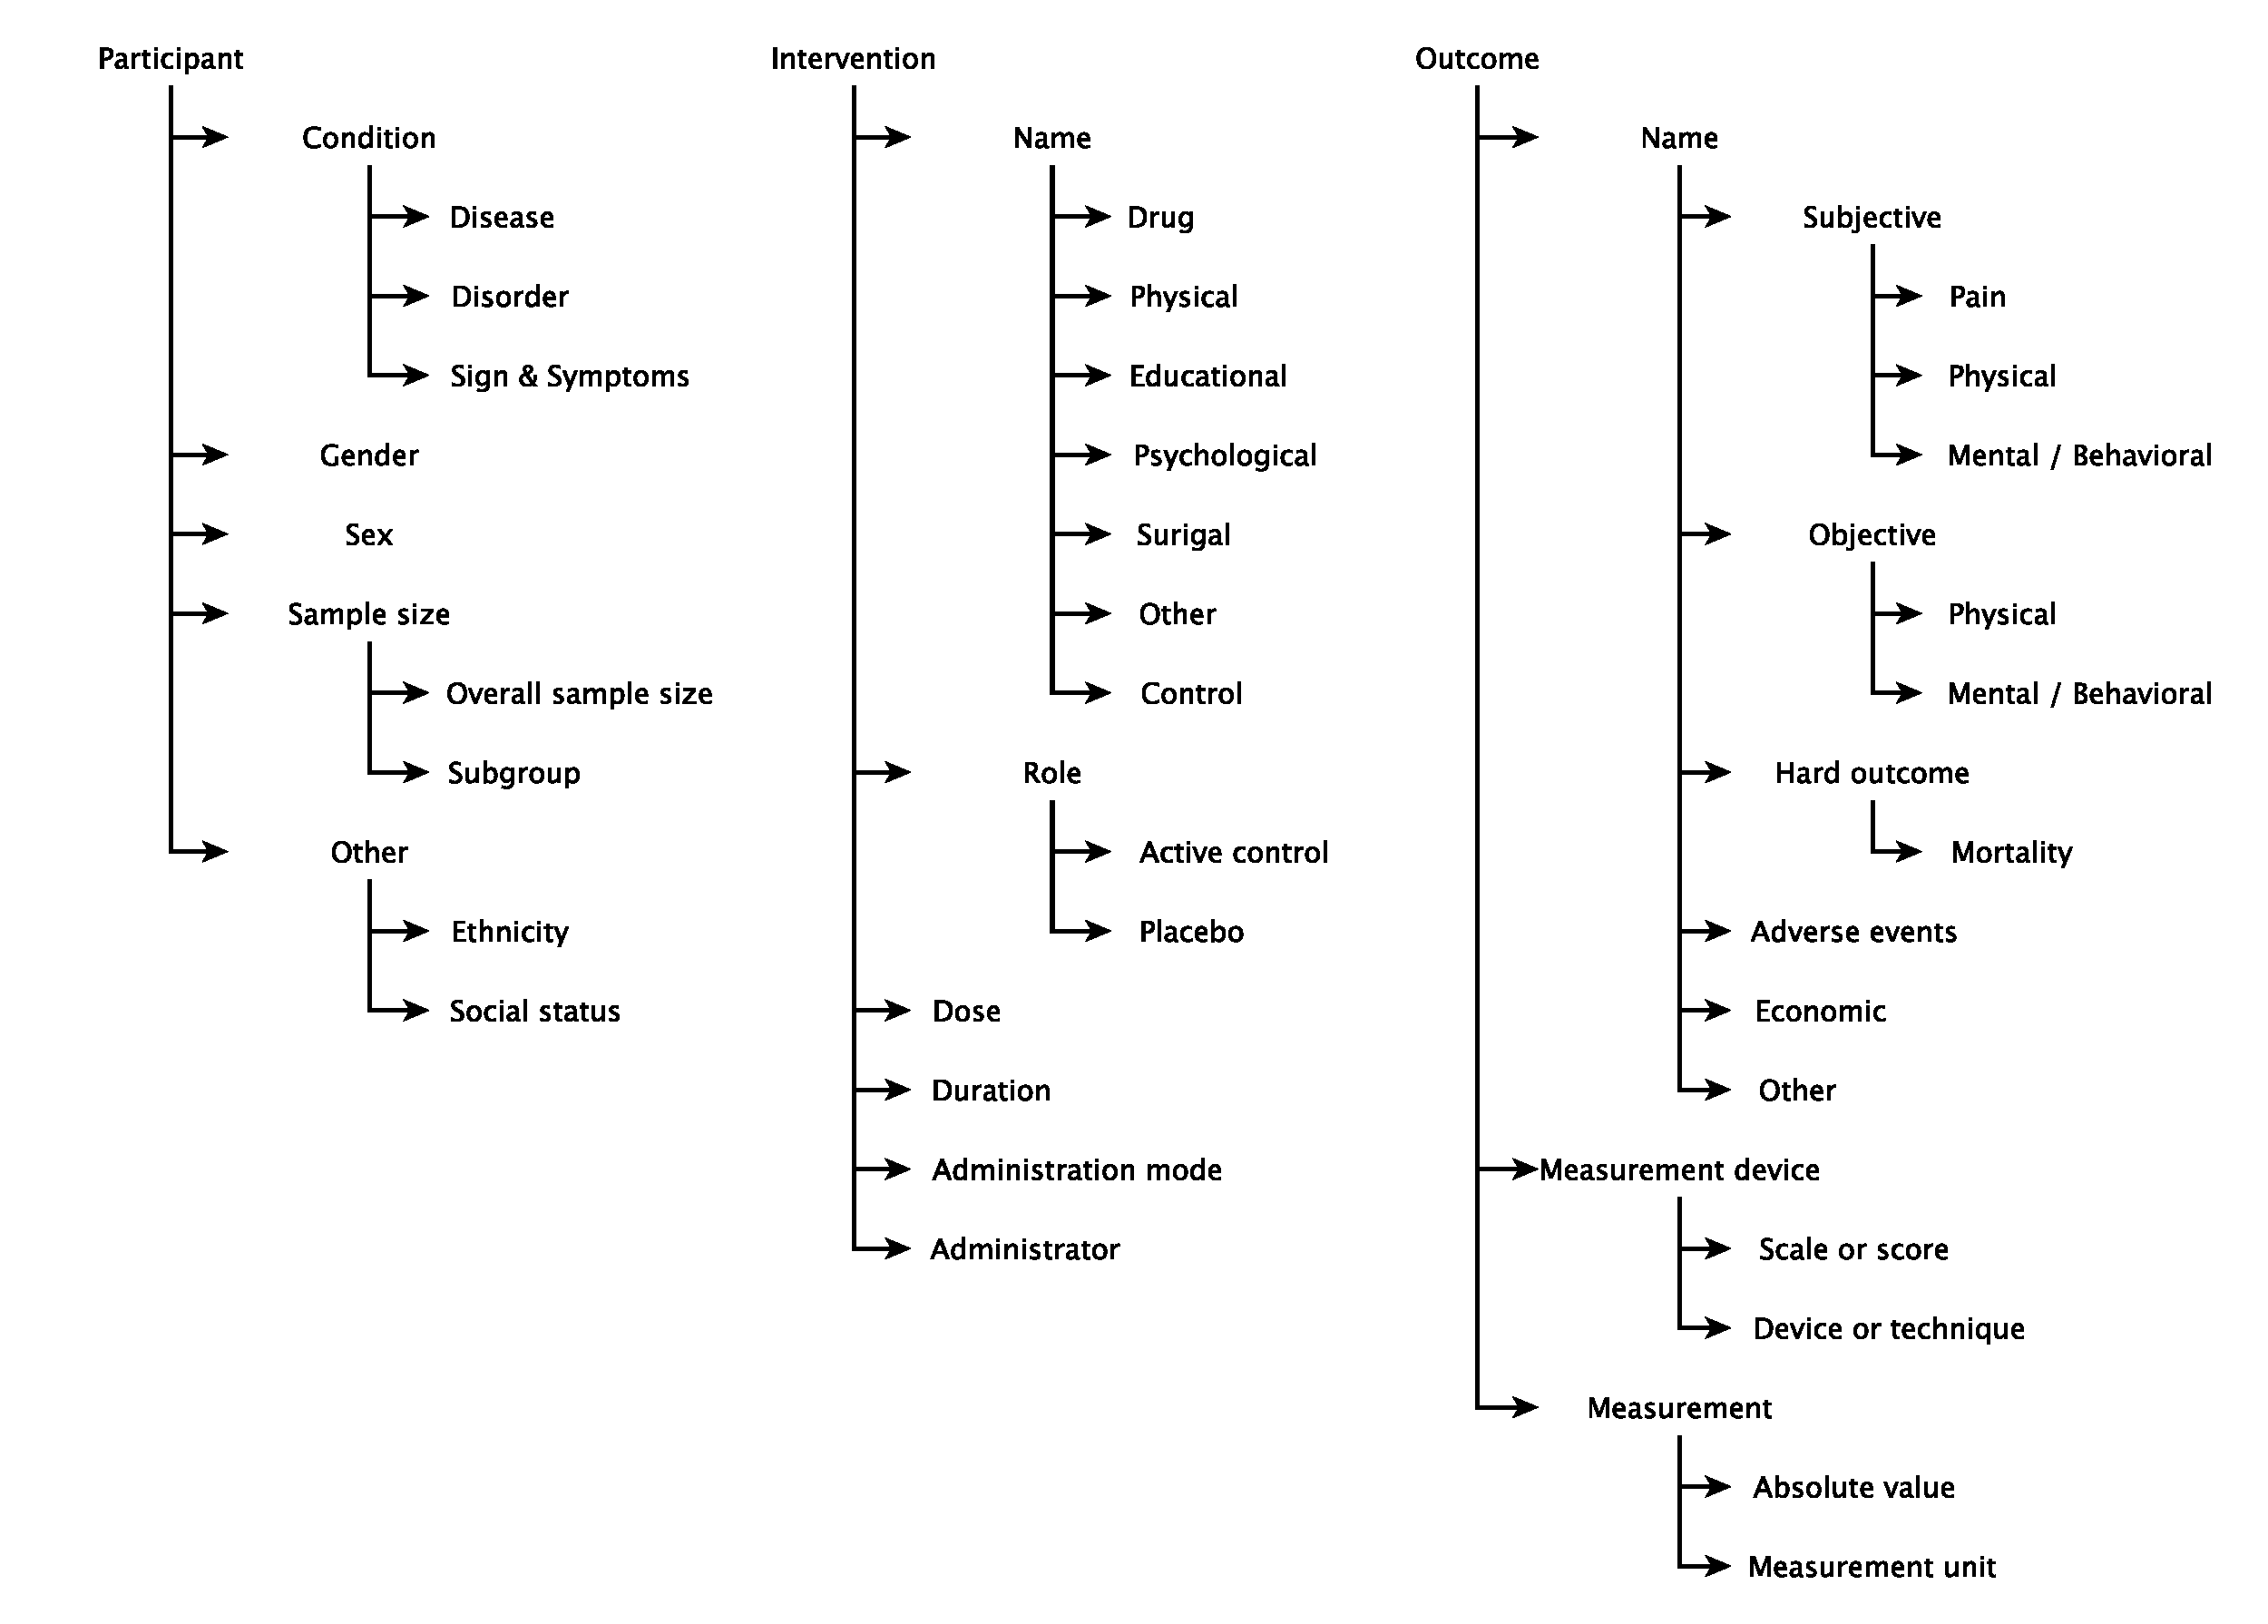
\includegraphics[width=0.95\textwidth]{figures/target_subgroups_.pdf}
\caption{\label{fig:target_subgroups} Hierarchical representation of PICO subclasses. The categories marked in bold italic are the same as the fine-grained categories in the EBM-PICO corpus.}
\end{figure}
%
%
%
\subsection{Error rectification}
%
We rectified the errors in the EBM-PICO validation subset and categorized them for each PI(C)O class, as shown in Table~\ref{tab:errordist}.
Of 12,960 (\textasciitilde1\% of 1,303,169) validation tokens evaluated to gauge the errors, 18.30\% of the intervention class tokens, 23.39\% of the participant class tokens and 20.21\% of the outcome class tokens were errors.
The error analysis was used to correct fine-grained annotation errors in the EBM-PICO test set, and both the EBM-PICO and its updated version were used for evaluation.
We were constrained with obtaining multiple annotators for the re-annotation to calculate inter-annotator agreement (IAA).
Therefore, we calculated Cohen's $\kappa_{new}$ between the original EBM-PICO gold set and our re-annotation over 200 documents and compared it to Cohen's $\kappa$ (see Figure~\ref{fig:agreement}) provided by the authors of the original corpus.\cite{nye2018corpus}
The 

%\paragraph{\textit{error rectification: impact}}
Table~\ref{tab:res} reports macro-averaged F1 for the experiments detailed in the experiments section compared to the fully-supervised approach.
Error rectification leads to an overall average F1 improvement of 4.88\% across the experiments using a weakly labelled training set with the highest average improvement of 8.25\% (7.15\%-9.52\%) for participants and 2.68\% (-0.11\%-4.28\%) for outcomes. 
For the participant class, both the LM and the WS F1 scores increase the full supervision score by 0.90\% - 1.71\%.
It has to be noticed that weak supervision outperforms full supervision on the rectified benchmark only for the participant entity.
%
\begin{table}[!ht]
    \centering
    \begin{tabular}{|l|r|r|r|}
    \hline
        Error category & Participant & Intervention & Outcome \\ \hline
        Repeat mention unmarked & 213 & 227 & 207 \\ 
        Remain un-annotated & 47 & 59 & 71 \\ 
        Inconsistency & 46 & 18 & 85 \\ 
        Punctuation/article & 15 & 23 & 48 \\ 
        Conjunction connector & 30 & 36 & 57 \\ 
        Junk & 53 & 79 & 30 \\ 
        Extra information & 80 & 146 & 58 \\ 
        Generic mention & 70 & 120 & 85 \\ \hline
        Total errors & 554 & 708 & 641 \\ \hline
    \end{tabular}
    \caption{\label{tab:errordist} Error distribution and error categories in the analysed tokens (\textasciitilde1\%) of EBM-PICO corpus.}
\end{table}
%
%
\begin{figure}[!h]
\centering
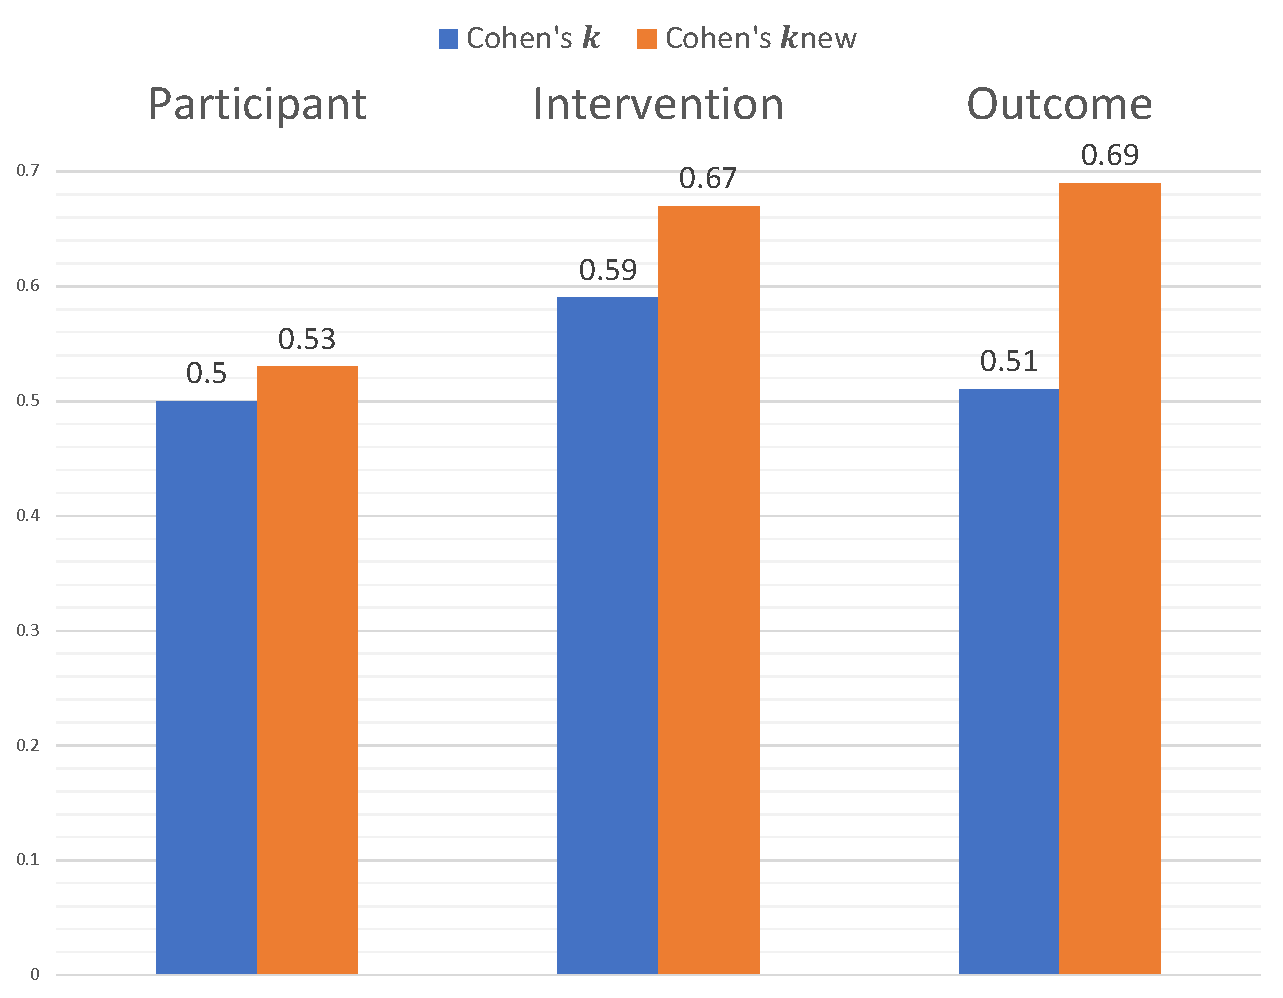
\includegraphics[width=0.65\textwidth]{figures/cohens_kappa.pdf}
\caption{\label{fig:agreement} Cohen's $\kappa_{new}$ between the expert annotated EBM-PICO gold test set and EBM-PICO compared to the Cohen's $\kappa$ for EBM-PICO gold test set annotations.}
\end{figure}
%
%
\begin{table}[!ht]
    \centering
    \begin{tabular}{|l|l|c|l|l|l|l|l|l|l|l|}
        \hline
        \multicolumn{3}{|c|}{} &
        \multicolumn{2}{|c|}{MV} & \multicolumn{2}{|c|}{LM} & \multicolumn{2}{|c|}{WS} & \multicolumn{2}{|c|}{FS} \\
        \hline
        Target & LF source & \#LF & Fine & Corr & Fine & Corr & Fine & Corr & Fine & Corr \\  \hline
        P & UMLS & 3-4 & 62.13 & 69.28 & 64.28 & 72.22 & 65.32 & 73.49 & 72.99 & 74.41 \\
         & +Ontology & 4 & 61.72 & 69.32 & 64.23 & 72.18 & 64.76 & 72.31 &  &  \\ 
         & +Rules & 19-119 & 63.08 & 72.06 & 65.79 & 75.31 & 66.73 & \underbar{\textbf{76.12}} &  &  \\ \hline
        I/C & UMLS & 8-95 & 59.7 & 63.94 & 60.11 & 64.28 & 59.17 & 61.72 & \textbf{83.37} & 81.06 \\ 
         & +Ontology & 5-101 & 62.14 & 66.92 & 62.83 & 67.09 & 67.06 & 69.76 & &  \\
         & +Rules & 4-35 & 58.51 & 63.45 & 64.34 & 68.17 & 70.27 & \underbar{72.39} &  &  \\ \hline
        O & UMLS & 5-6 & 55.79 & 59.85 & 58.76 & 62.36 & 60.83 & \underbar{63.55} & \textbf{81.2} & 80.53 \\
         & +Ontology & 4-5 & 56.006 & 59.64 & 59.27 & 62.34 & 59.55 & 60.46 &  &  \\ 
         & +Rules & 3-5 & 55.08 & 59.36 & 60.9 & 62.87 & 60.5 & 60.39 &  &  \\ \hline
    \end{tabular}
    \caption{ Macro-averaged F1 scores for UMLS, UMLS+other and rule-based weak supervision. Underlined values show the best score without manually labelled training data. Bold values show the best overall F1 score in any category. Note: Fine = EBM-PICO fine-grained annotations, Corr = EBM-PICO fine-grained annotations (EBM-PICO updated)}
    \label{tab:res}
\end{table}
%

%
\paragraph{\textit{MV vs. LM vs. WS}}
The label model improved the average performance by 2.74\% (0.17\%-5.83\%) compared to majority voting.
However, PubMedBERT did not guarantee improved performance across the targets leading to performance drops between 0.4 - 2.56\%.
Though the weakly-supervised PubMedBERT models did not always improve the performance compared to their label model counterparts, they had the best F1 score for each target class.
The majority voting had higher recall across experiments compared to precision, while LM focused on precision (see Figure~\ref{fig:precRecall}), making it a possible choice for recall-oriented PICO extraction tasks.
%
\paragraph{\textit{LF tiers}}
Adding non-UMLS LFs to the UMLS tier increases performance for the intervention target by an average of 4.48\%, but leads to performance drops for the participants and outcomes targets by 0.36\% and 0.64\%, respectively.
Adding task-specific LFs increased the overall F1 by a negligible 0.98\%.
Heuristics improved performance for the interventions LM by 11.1\%.
%
\paragraph{\textit{UMLS partitions}}
To investigate the optimal number of UMLS labelling functions required, we used the same methodology as in Trove, holding all non-UMLS and heuristics LFs fixed across all ablation tiers and computed performance across $s = ( 1, 2, \dotso , 127 )$ partitions of the UMLS terminology.
We noticed an increased performance for the first few partitions. However, We did not see the performance drop with a further increase in the participant and intervention target partition number.
Partitions with more than 100 LFs performed better.
This situation contrasts with Trove, where an increase in partitions leads to a drop in performance across targets (see Figure~\ref{fig:partitions}).
For the outcomes target, an increase in the number of partitions leads to an increased performance initially but a drop with a further increase in the partition numbers.
LM outperforms MV on training performance across the two targets and experiments except for the intervention target, where the MV model combining UMLS and additional ontologies outperforms LM.
The simple baseline collapsing UMLS into a single LF usually did not perform better than the others in UMLS partitions for any of the three experiment tiers (refer to the \#LF columns in Table~\ref{tab:res}).
%
\begin{figure}[!h]
    \centering
    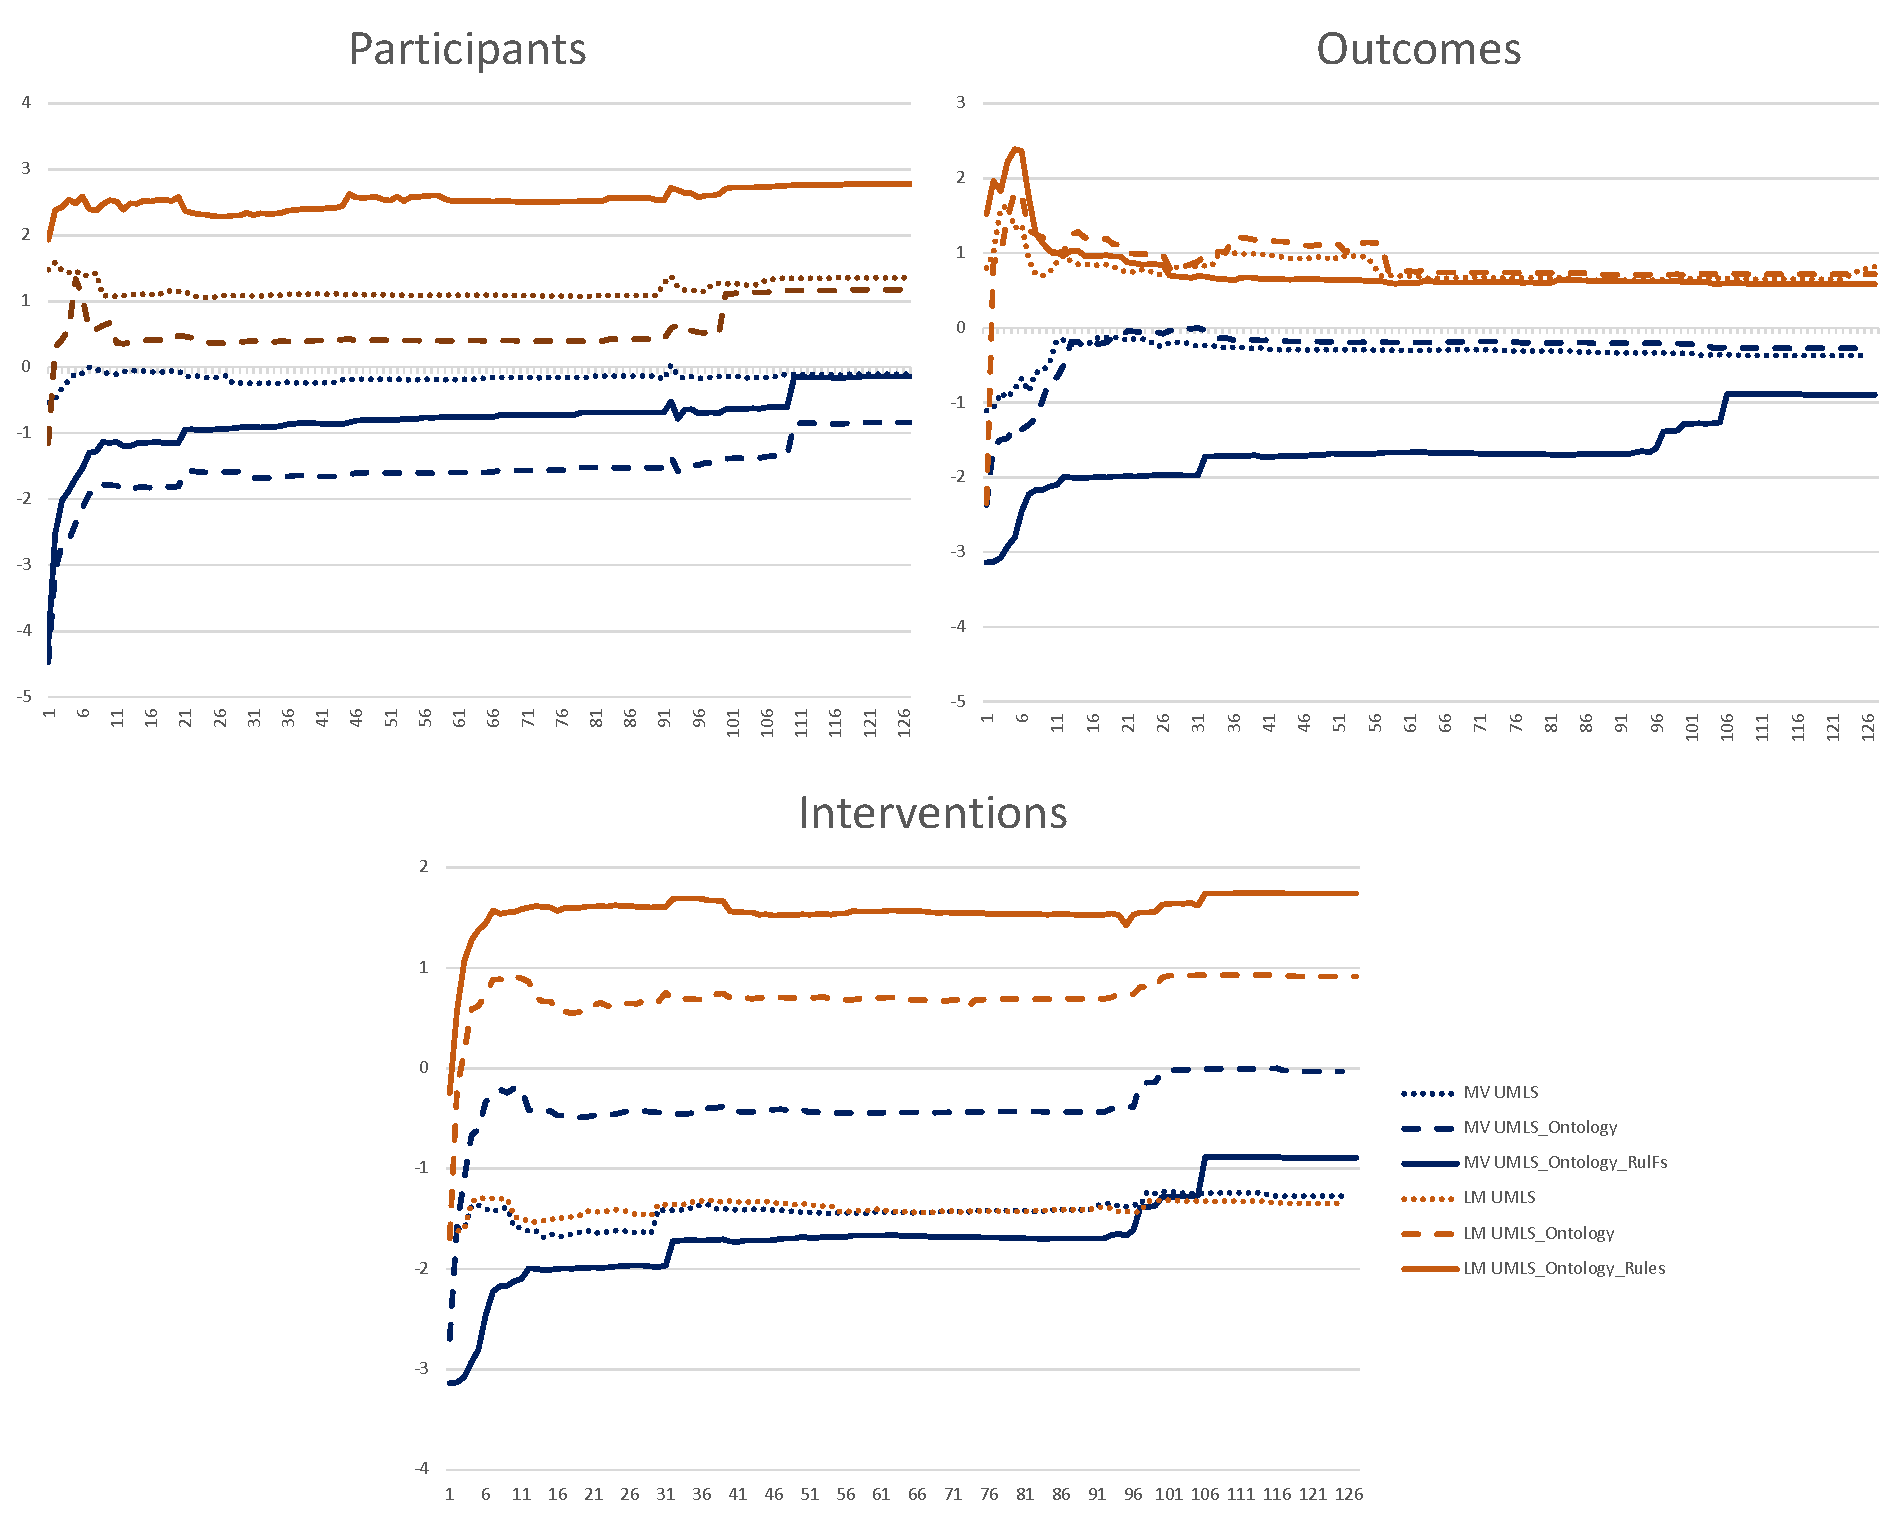
\includegraphics[width=0.95\textwidth]{figures/partitions.pdf}
    \caption{The relationship between the number of UMLS partitions and the macro-averaged F1 score for i) participants target, ii) interventions target and iii) outcomes target.}
    \label{fig:partitions}
\end{figure}
%
%
%
%==============================
\section{DISCUSSION}\label{discussion}
%==============================
%
Our study results show promising performance of weak supervision compared to full supervision and surpassing it for participant extraction.
It has to be noticed that weak supervision requires careful LF design consideration to surpass full supervision, primarily due to the compositional nature of PICO classes.
In another study, we use this weak supervision approach to successfully extend PICO to PICOS extraction (S = Study type) without needing additional annotated ``Study type'' data to quickly power applications.\cite{dhrangadhariya2023picos}


Although it is to re-purpose the vocabularies for pseudo-labelling, it is challenging to map them to the correct PICO targets.
A decreased or stagnant F1 after adding non-UMLS LFs to the UMLS tier indicates this.
We used the EBM-PICO validation set to design task-specific LF for all the PICO targets.
Still, the performance boost using these LFs was only observed in the participants and interventions and was detrimental to the outcomes.

Even though LM improves performance compared to MV, MV has a higher recall across experiments indicating a good corpus coverage of the LFs (refer to Figure~\ref{fig:precRecall}).
While some studies press on PICO extraction being a recall-oriented task, this is debated in practice.
In practice, high recall might lead to a high false positive (FP) rate, leading to the reviewers spending more time weeding out FP noise than reading and annotating the abstract with the entities.\cite{liu2021sent2span}


LM only considers the information encoded in the weak sources to label phrases from the training text but does not consider the contextual information.
Transformers consider the contextual information and should generalize beyond the label models in theory.
It is empirically confirmed by the performance boost that PubMedBERT brings this on top of the label model for some instances, but the weakly-supervised outcomes extraction results refute it.
%
\begin{figure}[!h]
    \centering
    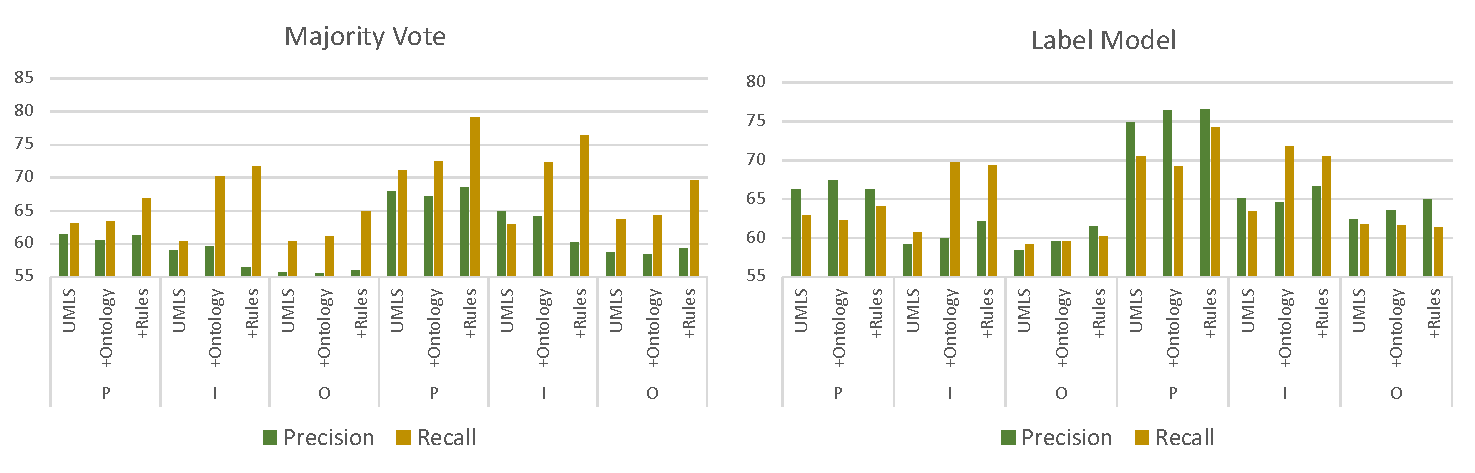
\includegraphics[width=0.99\textwidth]{figures/precRecall.pdf}
    \caption{Precision and recall across the experiments for the I. Majority vote models (left) and II. Label models (right)}
    \label{fig:precRecall}
\end{figure}
%
%
%
\subsection{Error analysis}\label{error_an}
%
Finally, we conducted an error analysis on 18 (n = 5,291 tokens) out of 200 EBM-PICO gold test set documents to gauge where weak supervision falters compared to full supervision.
Table\ref{tab:error_ner} shows token level errors divided into either of the four classes: 1) false negative (FN) - if the entire entity that the token was part of was missed out by the LM, 2) false positive (FP) - if the entire entity that the token was part of was falsely recognized as an entity, 3) boundary error (BE) - if the boundary tokens were missed out but otherwise the entity was identified by LM prediction, and 4) overlapping error (OE) - if LM made an error in the non-peripheral tokens of an otherwise identified entity mention.
Non-peripheral tokens are all tokens except the first and last of the multi-token entity.

We aim to improve recall for the weakly supervised PICO and thus dig deeper into the FNs.
Besides participant disease, many a time, tokens representing participant sample size, age group, gender, and symptoms subclasses went unrecognized.
The LM labelled these FNs with low confidence, meaning it picked up the signals from the LFs, although the signals were not strong enough for correct classification. 
Such FNs could be mitigated by weighting LFs for these subclasses.
Considerable standard and unusual abbreviation terms were missed out, especially the ones encompassed by brackets, e.g., MetS (Metabolic Syndrome), TC+TSE (testicular cancer + testicular self-examination), LVH (left ventricular hypertrophy), \textit{etc.}.
The model did not pick some of the standard abbreviations, e.g. LVH and MetS, due to a faulty mapping of these abbreviations to the incorrect PICO target.
A similar pattern was observed for the intervention (e.g., IBA (Inference-based Approach), RT (Radiotherapy)) and outcomes class abbreviations too.
The mismapping is now amended.
LM did not capture the abbreviations enclosed in a bracket (e.g., ``(COPD)'') as the LFs were not designed to tag these brackets.
BE FNs were usually the extra information that described more about the participant's disease, e.g., the information about disease staging went unrecognized in the participant's disease entity (in ``advanced carcinoma'', the word ``advanced'' was a BE FN).

Intervention LMs did not recognize common drug names, e.g. Fenofibrate and CP-529,414.
In addition, many non-standardized treatment names went unrecognized, e.g. substance abuse prevention program, inference-based approach, high-concentration contrast agents, epigastric impedance, etc.
Such terms are absent from both UMLS and non-UMLS vocabularies leading to FNs, so the LFs do not encode them.
Similarly, BEs were the non-idiosyncratic tokens partially misrecognized because the vocabulary did not encode this partial information.
E.g., the term ``internal stenting'' is partially recognized because ``stenting'' is a UMLS concept but not ``internal''.
Similarly, in the term ``endopyelotomy stent placement,'' only the UMLS concept token ``stent'' was identified.
Such entities not encoded by the LFs contribute to the FNs and could be mitigated by adding relevant vocabulary and rules.\cite{augenstein2017generalisation}

%The study intervention ``cholesteryl ester transfer protein'' was possibly missed because this UMLS concept fell under the ``Amino Acid, Peptide, or Protein'' semantic group, which was marked abstain for intervention.
It is straightforward to add vocabulary but challenging to map a semantic group to PICO categories, especially in the outcomes class.
Our current source-to-target mapping approach is manual and based on subjective expert judgment and could be improved by an objective algorithm.
This could have led to several spurious FPs, especially for the outcomes and to a less extent for the intervention class.
It also took time to identify semantic categories and UMLS vocabularies corresponding to the study outcomes pointing towards the gap in developing one.
%
\begin{table}[h!]
\begin{center}
\begin{tabular}{| c | c | c | c | c |} 
\hline
 & FP & FN & BE & OE \\ 
\hline
Participants & 160 & 76 & 80 & 10 \\ 
Interventions & 308 & 119 & 60 & 0 \\ 
Outcomes & 233 & 306 & 139 & 7 \\ 
\hline
\end{tabular}
\caption{\label{tab:error_ner} Distribution of the token-level errors made by the best label models on EBM-PICO gold.}
\end{center}
\end{table}
%
%
%
%==============================
\section{CONCLUSION}\label{conclusion}
%==============================
%
We adapted weak supervision for PICO spans and developed models for predicting PICO entities without a hand-labelled corpus.
We also identified errors pertinent to the current PICO benchmark, rectified them and used both datasets to evaluate the recognition models.
The approach achieves promising performance compared to full supervision and warrants further research into weak supervision for challenging PICO extraction.
The approach can be extended to more clinical SR entities without a manually labelled corpus, thereby being a starting point to overcome the annotation bottleneck.
In the future, we will work on extending the data programming approach to inspect strategies for objectively mapping ontologies to PICO subclasses and using external models like MetaMap as LFs.
%
%
%
%==============================
\section{ABBREVIATIONS}\label{abb}
%==============================
%
\begin{itemize}
    \item SR: Systematic Review 
    \item PICO: Participant, Intervention, Comparator, Outcome
    \item PICOT: Participant, Intervention, Comparator, Outcome, timeframe
    \item PICOS: Participant, Intervention, Comparator, Outcome, Study type and Design
    \item PIBOSO: Patients/Population, Interventions, Background, Outcome, Study Design, Other
    \item IO: Inside, Out
    \item RCT: Randomized Controlled Trial
    \item EBM: Evidence-based Medicine
    \item UMLS: Unified Medical Language System
    \item DO: Disease Ontology
    \item HPO: Human Phenotype Ontology
    \item OAE: Ontology of Adverse Events
    \item ChEBI: Chemical Entities of Biological Interest
    \item CTD: Comparative Toxicogenomics Database
    \item GSSO: Gender, Sex, Sexual Orientation Ontology
    \item NDD-CTO: Clinical Trials Ontology
    \item ONTOTOX: Chemotherapy Toxicities Ontology
    \item CCTOO: Cancer Care: Treatment Outcomes Ontology
    \item SYMP: Symptoms Ontology
    \item NPI: Non-pharmaceutical Interventions Ontology
    \item NCCO: Nursing Care Coordination Ontology
    \item NLP: Natural Language Processing
    \item WS: Weakly Supervised
    \item FS: Fully Supervised
    \item MV: Majority Vote
    \item LM: Label Model
    \item LF: Labelling Function
    \item NER: Named Entity Recognition
    \item NLTK: Natural Language Toolkit
    \item P: Participant
    \item I/C: Intervention/Comparator
    \item O: Outcome
\end{itemize}
%
%
%
%==============================
\section{ACKNOWLEDGEMENTS}\label{acknowledgements}
%==============================
%
The authors thank Dr Jason A. Fries for his valuable comments and insights on the labelling function design and label model execution phase of the study.
We thank in advance the anonymous reviewers for their time and feedback.
%
%==============================
\section{CONFLICT OF INTEREST STATEMENT}\label{conflictinterest}
%==============================
%
The authors have no conflicts of interest to declare. 
%
%==============================
\section{FUNDING}\label{funding}
%==============================
%
HES-SO Valais-Wallis, Sierre, Switzerland, funded the work.
%
%==============================
\section{ETHICS STATEMENT}\label{ethic}
%==============================
%
Our study focuses on the applicability of weak supervision for information extraction using publicly-available datasets.
Our investigation neither introduces any social or ethical concerns.
We do not foresee any direct social consequences or ethical issues.
%
%
%
%
%==============================
\section{DATA AVAILABILITY}\label{abb}
%==============================
%
The code is available on GitHub (\url{https://github.com/anjani-dhrangadhariya/distant-PICO}) and will be made public upon publication.
The EBM-PICO error analysis file for the validation set, the error-rectified EBM-PICO gold test set and other resources like distant supervision CTO dictionaries and hand-crafted dictionaries are available on Zenodo (DOI: 10.5281/zenodo.7320321). 
More information could be found in the supplementary file.
%
%
%
%Where the bibliography will be printed
%==============================
\printbibliography
%
%\bibliography{literature}
%==============================
%
%
%
\end{document}